
\documentclass{article}
\usepackage{amsmath, amsfonts, amssymb, amsthm} %packages for math-related
\usepackage[margin=1.2in]{geometry}
\usepackage[shortlabels]{enumitem}
\usepackage[utf8]{inputenc}
\usepackage{graphicx} % package for inserting images
\usepackage{commath} % package for things like \del, \cbr, and \sbr. These handle parentheses well.
\usepackage[mathscr]{euscript}%for \scr command 
\usepackage{../commands} %package with all of the commands for this class
\usepackage{url}
\setlength{\parindent}{0em} % so paragraphs aren't indented
\newcommand{\lcm}{\text{lcm}}
\newcommand{\Hom}{\text{Hom}}
\newcommand{\Ann}{\text{Ann}}
\newcommand{\Cc}{{C_c^\infty(\RR)}}
% ********************************************************** %
%               THINGS TO EDIT BELOW THIS LINE               %
% ********************************************************** %
\newcommand{\D}{\nabla}
\renewcommand{\d}{\partial}
\usepackage{wrapfig}
\title{\textsc{MATH 173 Problem Set 9}}
\author{Stepan (Styopa) Zharkov}
\date{June 1, 2022}
\begin{document}
\maketitle
\problem{1} 
\tri
\hop 
\solution 
Recall that we defined $G(x,y) = E(x-y) - \phi^x(y)$ where $\Delta \phi^x = 0$ and $\phi^x |_{\d
\Omega} = E(x - \cdot)$. So, if $Q(x,y) := G(x,y) - E(x-y) = -\phi^x(y)$, then $Q|_{\d(\Omega \times \Omega)} = -E(x-y)$ and $\Delta Q =0$. So, by the maximum principle, the minimum is achieved on the boundary. But the boundary is nonnegative, so  $Q> 0$, so $G(x,y) \ge E(x-y)$. \qed

\newpage
\problem{2} 
\tri
\hop 
\solution
\begin{enumerate}[(a)]
    \item We need $\intzo |x^\alpha|^2 = \intzo x^{2\alpha}$ to converge. This converges for $\alpha > -1/2$ and diverges for $\alpha \le -1/2$, so $\phi_\alpha \in L^2((0,1))$ for $\alpha > -1/2$. \qed
    \item We need $\phi_\alpha \in L^2((0,1))$, so $\alpha > -1/2$. But, since $\phi_\alpha$ are smooth, we also need $\intzo |\phi_\alpha ' |^2$ to converge. We see $\phi_\alpha' = \alpha x^{\alpha-1}$. and $\intzo |\alpha x^{\alpha-1}|^2 = |\alpha|^2\intzo x^{2(\alpha-1)}$ converges for $\alpha > 1/2$ and diverges for $\alpha \le 1/2$. So, $\phi_\alpha \in H^1((0,1))$ for $\alpha > 1/2$. \qed
\end{enumerate}

\newpage
\problem{3} 
\tri
\hop 
\solution
\begin{enumerate}[(a)]
    \item We know the statement is true for $f \in C^1((a,b))$ by FTC. Now, let $f_n \to f$ where $f_n \in C^1((a,b))$. By the continuity of the trace operator, 
    \[f(y) - f(x) = \limty (f_n(y)-f_n(x)) = \limty \int_x^yf_n'(t)dt\]
    Now, since we are on a bounded interval, we can move the limit inside the derivative after applying dominated convergence to see that 
    \[\limty \int_x^yf'_n(t)dt - \int_x^yf'_n(t)dt = \limty \int_x^y(f_n(t) - f(t))'dt = 0.\]
    So, 
    \[f(y) - f(x) =  \int_x^yf'(t)dt\]
    as we wanted. \qed
    \item By Cauchy-Schwartz and part (a) and that $|f'|$ is bounded by $C$, 
    \begin{align*}
        |f(y) - f(x)|^2 &= |\int_x^y f'(t)dt|^2\\
        &\le \int_x^y|f'(t)|^2 dt \\
        &\le \int_x^yC^2 dt \\
        &= |y-x|C^2.
    \end{align*}
    So, $|f(x) - f(y)| \le C|x-y|^{1/2}$. \qed
\end{enumerate}

\newpage
\problem{4} 
\tri
\hop 
\solution First, note that for $f \in C^1((a,b))$ where $f(a)= f(b)= 0$, and any $x \in (a,b)$, we have by Cauchy Schwartz,
\begin{align*}
    2||f||_2||f'||_2 &= 2\del{\int_a^b|f(t)|^2}^{1/2}\del{\int_a^b |f'(t)|^2}^{1/2}\\
    &\ge 2\int_a^b |f(t)f'(t)|dt \\
    &\ge 2\int_a^x |f(t)f'(t)|dt \\
    &\ge \abs{\int_a^x 2f(t)f'(t)dt} \\
    &= \abs{\int_a^x (f(t)^2)'dt} \\
    &= |f(x)^2 - f(a)^2|\\
    &= |f(x)^2|.
\end{align*}
Since $x$ was arbitrary, \[\sup_{(a,b)} |f(x)|^2 \le 2||f||_2||f'||_2.\]
Now, problem 3(b) and the fact that $H_0^1((a,b)) \sse H^1((a,b)) \sse C([a,b])$ gives us the same inclusion argument as in chapter 9.1, leading us to conclude the statement for all $f \in H^1((a,b))$. \qed

\newpage
\problem{5} 
\tri
\hop 
\solution Consider the dogbowl functions 
\[f_n := 1-\min(n\cdot d(x, \d B), 1).\]

\image{4cm}{dogbowl}

We see that $Tf_n = 1$ for all $n$, so $Tf_n \to 1 \ne 0$. However, 
\[||f_n||_{L_2}^2 = \int_B |f_n(x)|^2dx = \int_{d(x,\d B)< 1/n} |f_n(x)|^2dx \le  \int_{d(x,\d B)< 1/n} 1 dx  = O(1/n) \to 0.\]
So, $f_n \to 0$ in $L^2$. \qed
 
\newpage
\problem{6} 
\tri
\hop 
\solution Let $u = \limty u_n$ where $u_n$ are compactly supported continuous functions. Note that we are given that $u = \limty -u_n(x^*)$. This means that 
\[u = \frac{ \limty u_n(x) + \limty -u_n(x^*)}{2}= \limty \frac{u_n(x)-u_n(x^*)}{2}.\]
Note that $\frac{u_n(x)-u_n(x^*)}{2}= 0$ when $x_n =0$, so 
\[T_{B_+}\del{\frac{u_n(x)-u_n(x^*)}{2}} =\frac{u_n(x)-u_n(x^*)}{2}|_{\d B_+} = 0.\]
We have shown in class that this is sufficient to say $T_{B_+}(u|_{B_+}) = 0$, so $u|_{B_+}\in H_0^1(B_+)$. \qed

\newpage
\problem{7} 
\tri
\hop 
\solution
\begin{enumerate}[(a)]
    \item Let $V_k = \{x : |x| < 1/k\}$ and let $W_k =\{x: 1- 1/k < |x| < 1\}$. Then, consider lemonsqueezer functions $f_k \in $ such that $f \in C_0^1(U)$ and $f_k|_{B(V_k \cap W_k)} = 1$ and $f_k|_{V_{2k} \cup W_{2k}} = 0$ with $O(k)$ derivatives. 
    
    \image{4cm}{lemonsqueezer}

    Note that $u_k := uf_k \in C_0^1(U)$. We claim $u_k \to u$ in $H^1(B)$. Note that 
    \[||u-u_k||_{H^1}^2 = \int_B|u - u_k|^2+ \int_B|\D u -\D u_k|^2.\] 
    Now, since $u$ is bounded
    \begin{align*}
        \int_B |u - u_k|^2 &= \int_B|u|^2|1-f_k|^2 \\
        &= \int_BO(1)|1-f_k|^2 \\
        &=O(1) \int_B|1-f_k|^2 \\
        &=O(1) \int_{V_k \cup W_k}|1-f_k|^2 \\
        &=O(1) \int_{V_k \cup W_k}O(1) \\
        &=O(1/k^n)=o(1)
    \end{align*}
    where the asymptotic notation is with respect to $k$.
    Also, 
    \begin{align*}
        \int_B|\D u -\D u_k|^2 = \int_B|\D u -\D u f_k - u \D f_k |^2 \le 2\int_B|\D u|^2 |1-f_k|^2 + 2\int_B|u \D f_k|^2.
    \end{align*}
    Note that since $|\D u|$ is bounded, applying our above logic to the first part gives us 
    \[2\int_B|\D u|^2 |1-f_k|^2 = O(1) \int_B|1-f_k|^2 = o(1).\]
    So, we only need to deal with the second part. We see that since $u$ is bounded and $\D f_k$ is mostly 0,
    \begin{align*}
        2\int_B|u \D f_k|^2 &=  2\int_B|u|^2|\D f_k|^2\\
        &= O(1)\int_B |\D f_k|^2 \\
        &= O(1)\int_{V_k \cup W_k}|\D f_k|^2 \\
        &= O(1)\int_{V_k \cup W_k}|O(k)|^2 \\
        &= O(1) O(1/k^n) O(k^2) \\
        &= o(1)
    \end{align*}
    for $n > 2$. Thus, combining everything, we see that 
    \[||u-u_k||_{H^1}^2 = o(1),\]
    which is what we needed to show that $H_0^1(B) = H_0^1(U)$. \qed
    \item Consider $u(x) = 1- x^2 \in C^1((-1,1))$. Note that $T_{(-1,1)} u = 0$, so $u \in H_0^1((-1,1))$. However, $T_{(-1,0) \cup (0,1)}u \ne0 $ so $u \not \in H_0^1((-1,0) \cup (0,1))$. Thus, 
    \[ H_0^1((-1,1)) \ne H_0^1((-1,0) \cup (0,1))\]
    \qed
    \item Note that the logic in part (a) does not go through with $n=2$ because we get $O(1)$ where we need $o(1)$. To fix this, it suffices to pick a different set of $f_k$ and it turns out that $H_0^1(B) = H_0^1(U)$ for two-dimensional balls. The problem is that our $f_k$ were interesting (nonflat) on a quickly shrinking region, so the derivative was forced to be large. 
    \hop
    So, instead we will make the $f_k$ interesting on a nonshrinking region. Keeping it linear will not work because we need it to still approach 1 quickly. So, consider the following set of lemonsqueezer functions:
    \hop 
    Let $c$ be a constant less than $1/\sqrt{2}$. Let $a_k$ be a quickly decreasing sequence. Now, let $f_k$ be constant 0 inside the square of sidelength $2a_k$ around the origin. Let $f_k$ be constant 1 outside the square of sidelength $2c$ but outside of $W_k$. Let the outer edge be smoothed out to 0, as in part (a). For the square in the middle, let each side follow the function $1 - (1-r/c)^{k}$ where $r := \min(|x-a_k|, |y-a_k|)$. We can smooth out the edges on arbitrarily small areas later. So, our picture looks something like this: 

    \begin{center}
        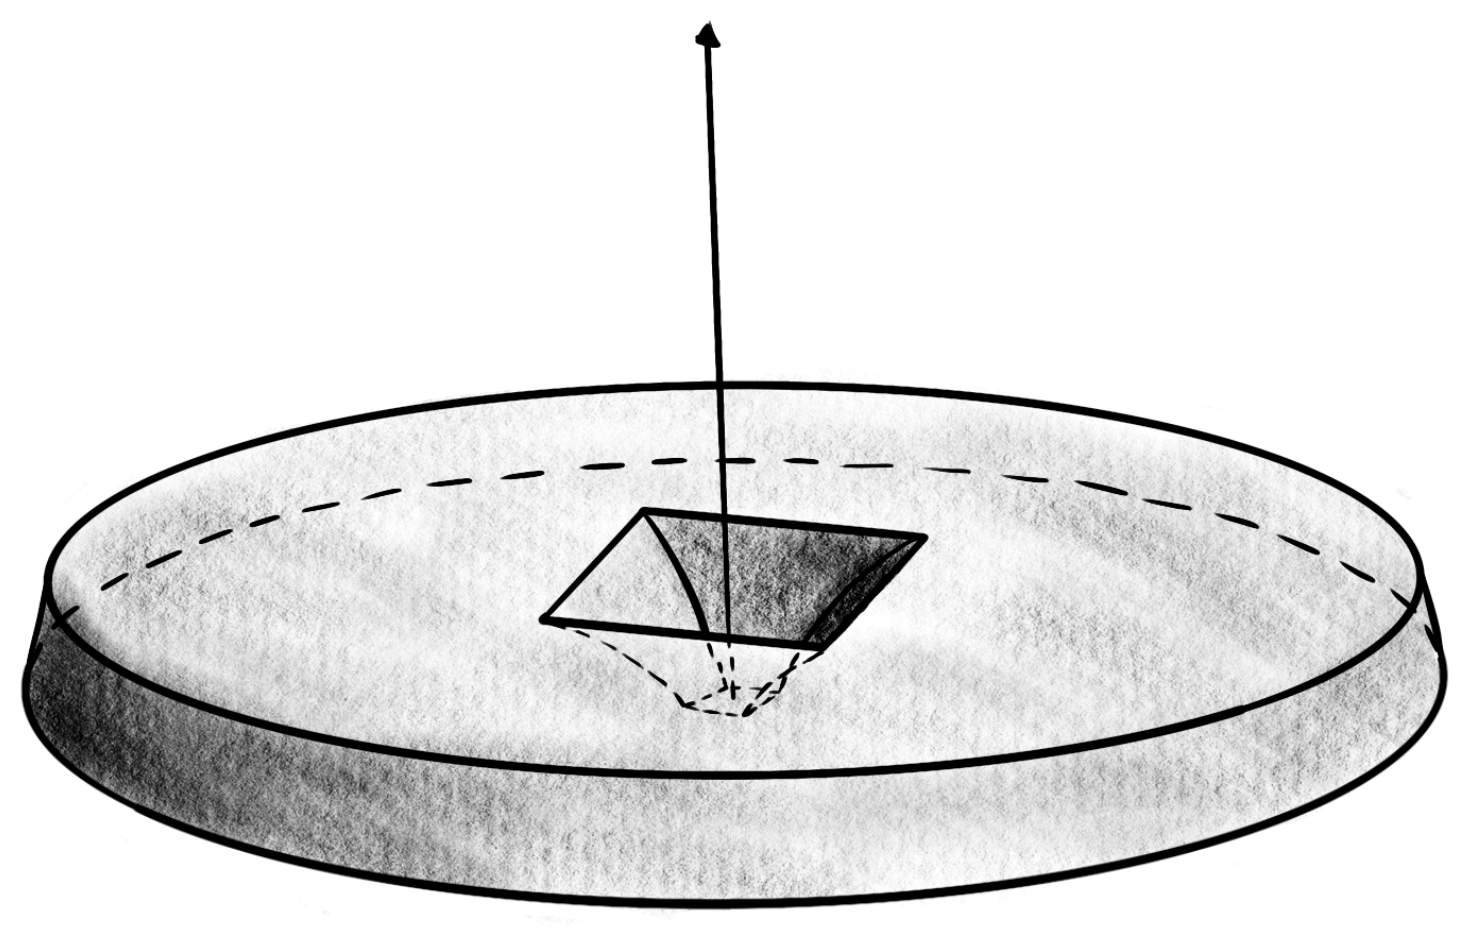
\includegraphics[height=3cm]{../images/lemon1}
    \end{center}

    \begin{center}
        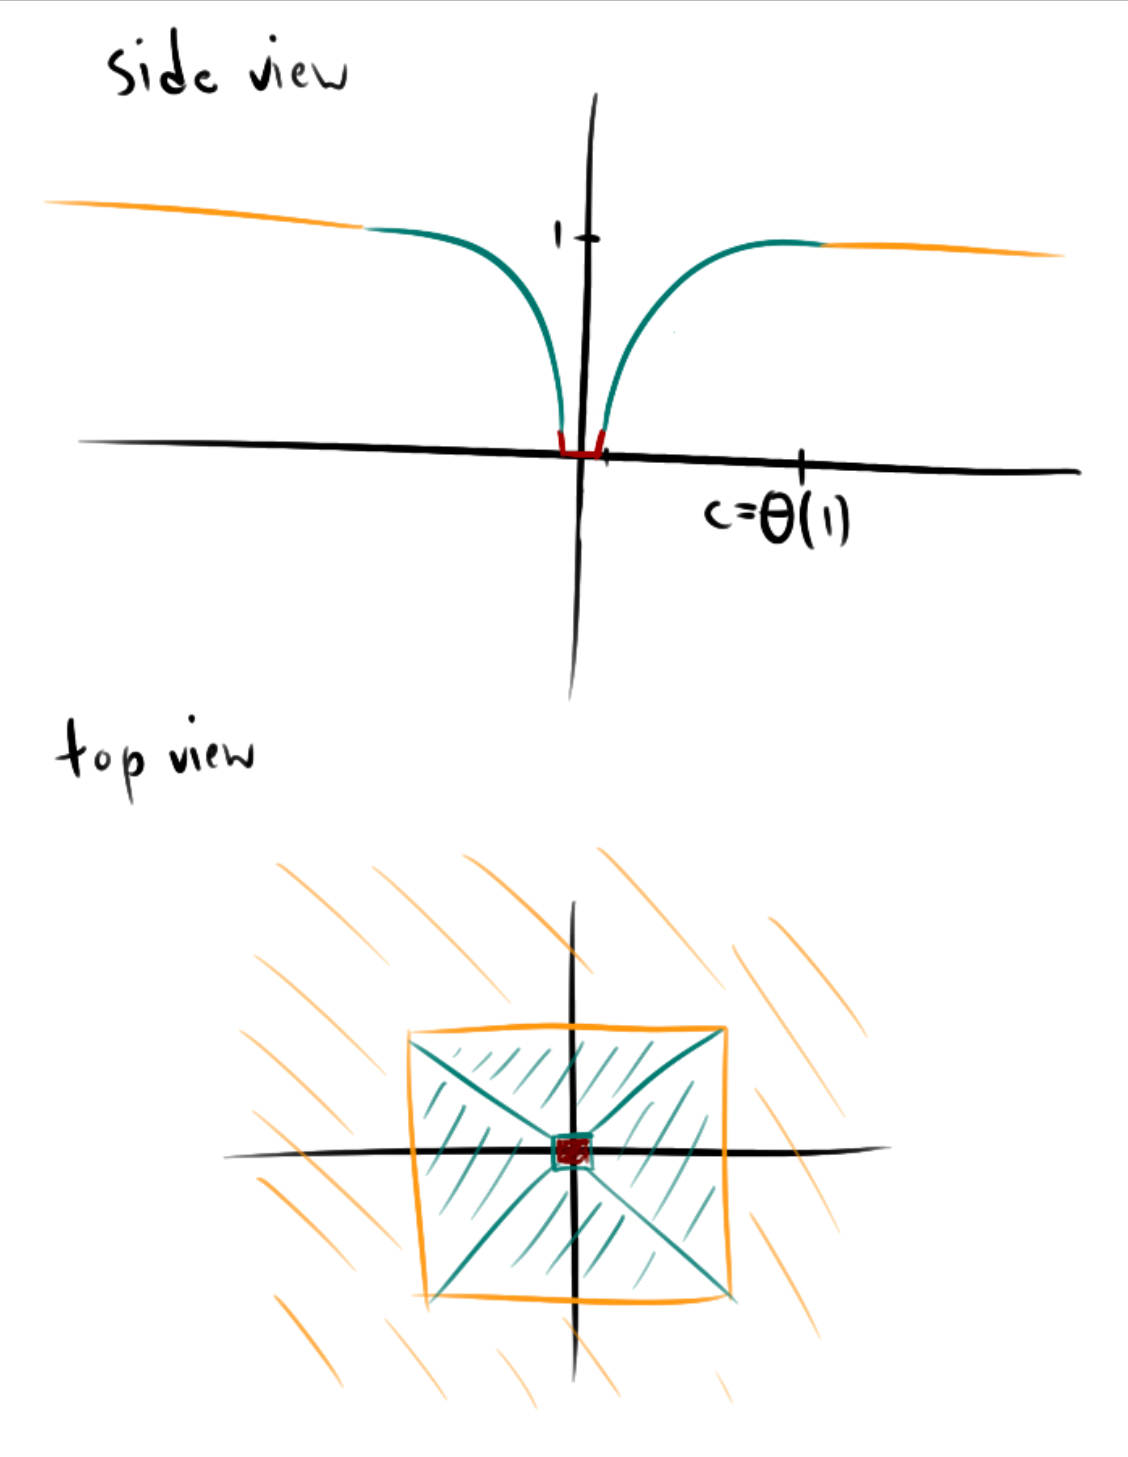
\includegraphics[height=6cm]{../images/lemon2}
    \end{center}

    Note that all of the steps in part (a) go through the same for $n=2$ except for bounding 
    \[\int_B|u \D f_k|^2.\]
    Since $u$ approaches 0, on the edges, we only have to worry about what happens in the center. 
    \[\int_{x,y: r < c-a_k}|u \D f_k|^2.\]
    % We can approximate $u$ by a sequence of functions that are flat around the origin. Selecting $k$ large enough that $c_k$ fits inside the flat region, we can assume that $u$ is constant in the region $\{x,y: r < c_k - a_k\}$. We will abuse notation by calling $u$ the value of $u$ at 0. 
    We see that since $u = O(1)$ and $|\D f_k| = O(k)(1-r/c)^{k-1}$, we can split the area into 8 triangles to see
    \begin{align*}
        \int_{x,y : r < c-a_k}|u \D f_k|^2 &= O(1) \int_{x,y : r < c-a_k}|\D f_k|^2 \\
        &=  O(1)\int_{x,y : r < c-a_k} O(k)(1-r/c)^{k-1} \\
        &= O(1)\int_0^c\int_0^x O(k^2)(1-r/c)^{2k-1} dydx \\
        &= O(k)\int_0^c\int_0^x (1-r/c)^{2k-2} drdx \\
        &= O(k)\int_0^c\int_0^x (1-r/c)^{\Theta(k)} drdx \\
        &= O(k)\int_0^c\int_0^x (1-r/c)^{\Theta(k)} drdx \\
        &= O(k)O(k\inv)\int_0^c (1-x/c)^{\Theta(k)} dx \\
        &= O(k)O(k\inv)O(k\inv)\\
        &= o(1).
    \end{align*}
    Thus, combining this with the rest of the reasoning from part (a), we have that 
    \[||u-u_k||_{H^1}^2 = o(1),\]
    completing the proof. \qed

\end{enumerate}
\end{document}